\documentclass[runningheads]{llncs}

\usepackage[T1]{fontenc}
\usepackage{graphicx}
\usepackage{hyperref}
\usepackage[style=numeric,backend=biber]{biblatex} % Utilisation de biblatex pour les références
\addbibresource{sample.bib}

\title{PER2024-010 - Identification de concepts dans les features apprises par un classificateur d'images}

\author{Guillaume ARRIGONI\inst{1} \and Timothée JUILLET\inst{1}}

\institute{Polytech Nice Sophia - Université Côte d'Azur, France \\
\email{guillaume.arrigoni@etu.univ-cotedazur.fr,timothee.juillet@etu.univ-cotedazur.fr}}

\begin{document}

\maketitle
\pagestyle{plain}

\begin{abstract}
Le cadre de ce projet est l'explication des décisions d'algorithmes de classification d'images par les différentes parties "conceptuelles" reconnues. Par exemple, on peut reconnaitre un chat par ses moustaches, ses oreilles, le fait que c'est un quadrupède, qu'il n'a ni ailes ni nageoires… Dans ce PER, on se basera initialement sur les travaux \autocite{binder2016layerwiserelevancepropagationneural} et \autocite{Achtibat2023} qui proposent chacun des méthodes différentes pour expliquer la décision de classification par des concepts. Les auteurs de \autocite{binder2016layerwiserelevancepropagationneural} proposent une méthode permettant d'établir les pixels les plus importants pour la décision du modèle en retro-propageant des scores de relevance à travers le modèle. \autocite{Achtibat2023} améliore cette méthode en permettant de restreindre cette rétropropagation de la relevance à une sous-partie du réseau (ie un sous-réseau): ceci permet de vérifier le lien entre des repères visuels (ailes, ...)  et des groupes de features associées (par une autre méthode) à des repères visuels. Des travaux préliminaires nous encouragent à étudier si l'étude des repères visuels liés à des sous-groupe de features permettrait d'identifier (sans autre méthode) des concepts dans un réseau de neurone.\par
Dans ce projet nous souhaitons établir une méthode permettant d'identifier des groupes de features associés à différents concepts et la transférabilité de ces groupes entre différents types d'images (canard -> crocodile). Pour ce faire, nous pourrons nous inspirer aussi d'autres travaux comme \autocite{9086075} proposant la construction (très coûteuse) d'un graphe pour l'explication hiérarchique d'une décision par les différentes parties d'un objet (e.g. c'est un cheval qui possède une tête de cheval, elle-même composée d'un museau, oreilles…) avec une relation de localisation relative entre éléments dont la sémantique semble partagée par toutes les images, contrairement à \autocite{binder2016layerwiserelevancepropagationneural,Achtibat2023}.

\end{abstract}

\textbf{Superviseur :} Frédéric Precioso (Polytech Nice Sophia, INRIA)


%\tableofcontents
\newpage

\section*{Remerciements}

Nous tenons à exprimer notre profonde gratitude à toutes les personnes qui ont contribué à la réalisation de ce Projet Encadré de Recherche.

Tout d’abord, nos sincères remerciements à M. Frédéric Precioso, notre encadrant principal, pour ses précieux conseils, son accompagnement bienveillant et son expertise, qui ont été essentiels tout au long de ce travail.

Nous remercions également Mme Diane Lingrand, notre co-encadrante, pour son aide précieuse et ses suggestions pertinentes, qui ont enrichi notre réflexion et ont permis d’améliorer la qualité de ce projet.

Enfin, nous souhaitons exprimer notre reconnaissance à M. Marco Winckler, responsable du PER, pour son engagement et son soutien dans l’organisation et le bon déroulement de ce travail.


\section{Introduction}

Ces dernières années, l'intelligence artificielle (IA) a connu des progrès spectaculaires, en particulier dans le domaine des réseaux neuronaux profonds (Deep Neural Networks, DNNs), qui ont permis des avancées majeures dans des applications telles que la reconnaissance d’images, la traduction automatique et les diagnostics médicaux. Cependant, la complexité des modèles rend leurs mécanismes internes opaques, soulevant des questions cruciales en termes de confiance, d’interprétation et de responsabilité, notamment dans des contextes sensibles comme la médecine. Pour répondre à ces enjeux, le domaine de l’Intelligence Artificielle Explicable (Explainable Artificial Intelligence, XAI) s’est développé, visant à rendre ces systèmes plus compréhensibles et transparents. Parmi les nombreuses applications de la XAI, une question particulièrement pertinente concerne l’explicabilité des modèles de classification d’images, un enjeu crucial dans des domaines tels que la médecine ou la vision par ordinateur. 
\bigskip

C’est dans ce cadre que s’inscrit notre projet, dont l’objectif est d’explorer et de développer des méthodes permettant d’expliquer les décisions de classification d’images des modèles en s’appuyant sur les parties 'conceptuelles' reconnues. Par exemple, un modèle identifiant un chat pourrait baser sa décision sur des concepts tels que les moustaches, les oreilles ou le fait qu’il s’agit d’un quadrupède sans ailes ni nageoires. Cette démarche repose sur l’hypothèse que les représentations internes des modèles peuvent être décomposées en concepts consistants et utiles, qui reflètent les caractéristiques visuelles fondamentales des données d’entrée. En identifiant ces concepts, il devient possible d’offrir une interprétation claire des mécanismes décisionnels des réseaux neuronaux et de valider la pertinence des décisions dans des contextes critiques.
\bigskip

Au-delà de l’identification des concepts, notre approche cherche également à évaluer leur robustesse et leur transférabilité. Cela implique d’analyser si les concepts identifiés dans un modèle restent valides lorsqu’ils sont appliqués à d’autres ensembles de données ou à des catégories d’objets différents. Par exemple, un concept lié à la reconnaissance de "moustaches" dans des images de chats doit-il être redéfini lorsqu’il est appliqué à des images de lions ? Ces questions sont essentielles pour garantir que les concepts interprétés sont non seulement explicables, mais également généralisables et cohérents dans divers contextes d’application.
\bigskip

Concrètement, les résultats de ce travail ouvrent la voie à des applications pratiques dans l’optimisation et l’amélioration des modèles d’apprentissage profond. Par exemple, les concepts identifiés comme pertinents pourraient être exploités pour simplifier les modèles via des techniques telles que le pruning ou la quantization. Ces méthodes permettraient de supprimer les informations ou caractéristiques non pertinentes, en conservant uniquement les concepts jugés utiles et consistants pour les décisions du modèle. Une telle optimisation pourrait réduire la taille des modèles et améliorer leur efficacité tout en maintenant un haut niveau de performance.
\bigskip

Enfin, comme dit au début, ce travail pourrait également contribuer à améliorer la transparence et la fiabilité des systèmes d’IA dans des domaines critiques. Dans la médecine, par exemple, il deviendrait possible d’expliquer précisément pourquoi un modèle détecte une anomalie en associant ses décisions à des concepts médicaux interprétables, renforçant ainsi la confiance des praticiens. De manière plus générale, cette approche pourrait faciliter le développement de systèmes d’IA plus explicables, modulables et adaptables, ouvrant de nouvelles perspectives pour l’interaction entre humains et machines dans des environnements complexes et exigeants.

\section{Etat de l'art}

Dans le contexte de l’explicabilité de l’intelligence artificielle, plusieurs recherches ont été menées pour répondre aux enjeux liés à la compréhension des décisions des modèles d’apprentissage profond. Parmi ces travaux, certains se sont concentrés sur l’analyse des prédictions individuelles, tandis que d’autres ont exploré les concepts appris par les modèles dans leur ensemble. Parmi les approches fondatrices, on retrouve celle de Binder, A., Montavon, G., Lapuschkin, S., Müller, KR., et Samek, W. (2016) \autocite{binder2016layerwiserelevancepropagationneural}, intitulée « Layer-Wise Relevance Propagation for Neural Networks with Local Renormalization Layers », qui a établi un cadre théorique essentiel pour la propagation de pertinence par couches (LRP). Cette méthode constitue une référence fondamentale pour comprendre les mécanismes de décision des réseaux neuronaux.

La méthode LRP, vise à résoudre un problème central des réseaux neuronaux profonds : leur opacité. Bien que ces modèles aient démontré des performances remarquables dans des tâches comme la classification d'images, comprendre les caractéristiques spécifiques influençant leurs décisions reste difficile. LRP décompose les prédictions couche par couche, attribuant des scores de pertinence à chaque pixel pour visualiser les éléments influents via des cartes thermiques. Cette capacité est particulièrement utile dans des contextes nécessitant une transparence accrue, comme la médecine, où les décisions algorithmiques ont des implications critiques.

LRP repose sur deux règles principales pour propager la pertinence des neurones : la règle $\varepsilon$, qui introduit un terme stabilisateur pour éviter les instabilités numériques lorsque la somme des activations est proche de zéro, et la règle $\beta$, qui sépare les activations positives et négatives pour redistribuer la pertinence de manière plus précise. Ces règles permettent d'obtenir des cartes thermiques qui mettent en évidence les contributions des pixels ou des régions spécifiques à la prédiction finale. Cependant, bien que robustes pour des architectures standards, ces règles nécessitent des adaptations lorsque des couches non linéaires complexes, telles que les couches de renormalisation locale, sont impliquées. Ces dernières modifient la distribution des activations des neurones en fonction de leurs voisins, ce qui complique la rétropropagation de la pertinence \autocite{binder2016layerwiserelevancepropagationneural}.

Pour répondre à ces défis, Binder et al. ont proposé une extension de LRP basée sur une approche de développement de Taylor au premier ordre. Cette méthode approxime les activations des neurones dans les couches de renormalisation à l'aide de séries de Taylor, permettant une décomposition plus fine et précise de la pertinence entre les neurones connectés. Cette adaptation garantit que la pertinence est correctement attribuée même dans les cas où les interactions locales jouent un rôle majeur dans les décisions du modèle. Les expérimentations réalisées sur des ensembles de données comme CIFAR-10 et ImageNet démontrent l'efficacité de cette approche, notamment en termes de qualité des explications fournies par les cartes thermiques, qui se traduisent par une meilleure performance en termes de zone sous la courbe (AUC), un indicateur clé pour mesurer la pertinence des explications \autocite{binder2016layerwiserelevancepropagationneural}.

Ces contributions méthodologiques sont d'une importance capitale pour les applications pratiques, car elles permettent une interprétation plus fine et fidèle des décisions des modèles dans des architectures intégrant des couches non linéaires complexes. De plus, les résultats expérimentaux valident l'impact des pixels identifiés comme les plus pertinents sur la précision des modèles, soulignant ainsi la robustesse des explications fournies par LRP. En offrant une solution pour des couches de renormalisation locale, cette méthode élargit considérablement le cadre d'application de LRP, rendant cette approche encore plus pertinente pour les architectures modernes \autocite{binder2016layerwiserelevancepropagationneural}. S'appuyant sur ces fondements théoriques, des chercheurs ont par la suite développé des approches plus sophistiquées pour répondre aux défis croissants de l'explicabilité des réseaux neuronaux. Parmi ces avancées, la méthode de Concept Relevance Propagation (CRP) proposée par Achtibat et al. (2023) \autocite{Achtibat2023} se distingue par son approche novatrice combinant les principes de LRP avec une compréhension plus approfondie des concepts humains.
\bigskip

L'intelligence artificielle explicable se divise généralement en deux grandes catégories de méthodes : les approches locales, qui se concentrent sur l'explication de prédictions individuelles, et les approches globales, qui visent à comprendre les concepts appris par le modèle dans son ensemble. Les méthodes locales, comme les cartes de saillance ou Grad-CAM \autocite{Selvaraju_2019}, mettent en évidence les zones d'une entrée jugées pertinentes par le modèle, mais elles ne donnent que peu d'informations sur la nature des caractéristiques détectées. Par exemple, si une région d'une image est jugée importante pour une prédiction, ces approches ne permettent pas nécessairement de savoir si cette région représente une oreille, un museau ou un autre élément conceptuel. Les méthodes globales, en revanche, tentent d'identifier les concepts appris par un modèle, mais elles manquent souvent de précision pour relier ces concepts à des prédictions spécifiques. Cette dichotomie entre le "quoi" (les concepts) et le "où" (les zones pertinentes) limite leur utilité dans des scénarios nécessitant une compréhension fine et contextualisée des décisions des modèles.

Pour surmonter ces limitations, Achtibat et al. (2023) ont introduit la méthode de Concept Relevance Propagation (CRP), qui propose une approche hybride et complémentaire \autocite{Achtibat2023}. La CRP combine la Propagation de Pertinence par Couches (Layer-wise Relevance Propagation, LRP) avec des techniques conditionnelles pour décomposer les prédictions en concepts humains compréhensibles et localiser ces concepts dans les entrées. Dans une tâche de classification d'images, la CRP peut expliquer qu'une prédiction "chien" repose sur des concepts tels que "fourrure", "yeux" ou "queue", tout en localisant précisément ces éléments dans l'image. Cette capacité dépasse les méthodes traditionnelles, souvent limitées à des visualisations floues ou ambiguës.

Un des aspects les plus remarquables de la CRP est son caractère généraliste et non intrusif. Elle peut être appliquée de manière post-hoc à presque tous les modèles d'apprentissage profond, sans nécessiter de modifications de leur architecture ou de leur processus d'entraînement \autocite{Achtibat2023}. Cela la rend particulièrement intéressante pour analyser des modèles déjà entraînés dans des domaines critiques, comme la médecine ou les sciences, où une explicabilité rigoureuse est souvent une exigence réglementaire ou éthique. De plus, la méthode de Relevance Maximization (RelMax), associée à la CRP, permet d'identifier les exemples les plus représentatifs pour un concept donné en fonction de leur contribution réelle aux décisions du modèle. Cela dépasse les pratiques courantes consistant à maximiser les activations des neurones, une approche parfois non représentative des processus d'inférence réels. 

La méthode CRP offre de nombreux avantages pratiques pour l'analyse et l'interprétation des décisions des modèles d'apprentissage profond. Elle permet notamment de détecter les biais et comportements indésirables, tels que l’utilisation de corrélations artificielles ou non pertinentes, en analysant les concepts latents et leur rôle dans les décisions spécifiques du modèle \autocite{Achtibat2023}. Par exemple, dans des modèles de classification d'images, la capacité de la CRP à établir des liens explicites entre des concepts humains compréhensibles (comme "fourrure" ou "yeux") et des prédictions spécifiques s'avère précieuse pour valider la robustesse des modèles et identifier des lacunes potentielles. En rendant ces relations accessibles aux utilisateurs finaux, cette approche contribue à accroître la transparence et la fiabilité des modèles, en particulier dans des domaines critiques tels que la médecine ou les sciences, où les conséquences des décisions algorithmiques peuvent être graves. Toutefois, bien que la CRP fournisse une base solide pour comprendre et expliciter les mécanismes décisionnels des réseaux de neurones, elle présente certaines limitations pour notre projet \autocite{Achtibat2023}. Ces limites se manifestent notamment par la non-prise en compte des connexions résiduelles, ce qui peut nuire à une interprétation complète des interactions complexes au sein des modèles.

S'appuyant sur ces avancées fondamentales, d'autres chercheurs ont développé des approches complémentaires pour répondre aux défis spécifiques posés par certaines architectures de réseaux neuronaux. Parmi ces développements, la méthode AttnLRP se distingue comme une adaptation innovante particulièrement pertinente pour les architectures de transformers.
\bigskip

Dans la continuité des progrès apportés par la CRP, AttnLRP \autocite{pmlr-v235-achtibat24a} élargit ces principes aux architectures de transformers, qui posent de nouveaux défis en raison de leurs mécanismes d'attention. Contrairement aux approches traditionnelles de LRP, qui peinent à traiter adéquatement des fonctions comme le softmax ou la multiplication bilinéaire, AttnLRP propose des règles d'attribution spécifiques qui conservent la pertinence tout en réduisant les instabilités numériques. Cette méthode attribue la pertinence en décomposant les contributions des matrices de requêtes, de clés et de valeurs dans les mécanismes d’attention, permettant une attribution plus précise et fine. De plus, elle intègre une approche innovante pour gérer les couches de normalisation, comme le LayerNorm, en linéarisant leurs effets pour garantir une attribution fidèle et stable, essentielle pour une interprétation fiable des modèles transformers \autocite{pmlr-v235-achtibat24a}.

Les contributions méthodologiques d’AttnLRP sont particulièrement notables. Elle permet non seulement de fournir des attributions au niveau des entrées, mais aussi d’analyser les neurones latents au sein des représentations internes des transformers. Cette capacité ouvre la voie à des manipulations directes des neurones latents, permettant par exemple d’influencer les sorties du modèle en activant ou désactivant des neurones associés à des concepts spécifiques. Des expériences menées sur des modèles de pointe comme LLaMa 2 et Flan-T5 montrent qu’AttnLRP surpasse les méthodes existantes en termes de fidélité des explications et d’efficacité computationnelle. Par exemple, en désactivant un neurone lié à un concept de "froid", il est possible de modifier une sortie décrivant un "ours polaire" pour qu’elle évoque un "dessert sucré". Ce niveau de contrôle interactif sur les représentations latentes représente une avancée majeure dans le domaine de l’explicabilité des modèles \autocite{pmlr-v235-achtibat24a}.

L’applicabilité d’AttnLRP ne se limite pas à une meilleure compréhension des mécanismes d’attention dans les architectures transformers. Elle ouvre également des perspectives prometteuses pour les systèmes critiques où la transparence et la robustesse des décisions sont essentielles, comme dans la médecine ou les sciences économiques. En fournissant des explications fidèles et interprétables des prédictions des modèles, AttnLRP s'inscrit comme une avancée significative dans le domaine de l’explicabilité des modèles complexes, permettant non seulement d’interpréter mais aussi d’interagir avec les concepts latents pour influencer les résultats.

Cependant, malgré ses nombreuses contributions, AttnLRP présente certaines limites. Sa dépendance aux mécanismes spécifiques des transformers, ainsi que ses exigences en termes de calculs, peuvent limiter son applicabilité dans certains cas d’usage. De plus, la méthode peine encore à capturer les interactions complexes entre groupes de features et concepts latents dans des scénarios plus diversifiés, ce qui reste un défi à relever pour aller plus loin dans l’explicabilité des modèles complexes.
\bigskip

Les méthodes étudiées dans cet état de l’art illustrent les avancées significatives réalisées dans le domaine de l’intelligence artificielle explicable (XAI). Des approches comme la Layer-Wise Relevance Propagation (LRP), la Concept Relevance Propagation (CRP), ou encore AttnLRP, ont permis de mieux comprendre les mécanismes décisionnels des modèles d’apprentissage profond. Cependant, elles présentent toutes des limitations notables qui restreignent leur applicabilité et leur efficacité face aux défis actuels. En particulier, ces méthodes peinent à relier explicitement des groupes de caractéristiques latentes à des concepts visuels compréhensibles, à garantir la robustesse et la transférabilité de ces concepts entre différents contextes, et à proposer des mécanismes généralisables à des architectures complexes telles que les transformers.

La LRP, bien qu’efficace pour visualiser les contributions des pixels dans les architectures classiques, nécessite des adaptations coûteuses pour les couches complexes comme la renormalisation locale. La CRP, quant à elle, offre une avancée majeure en introduisant une interprétation conceptuelle des prédictions, mais elle manque de mécanismes robustes pour généraliser ces concepts à d'autres ensembles de données ou architectures. Enfin, si AttnLRP fournit une explicabilité innovante pour les transformers, elle reste limitée dans sa capacité à capturer des interactions complexes entre groupes de concepts et à gérer efficacement la diversité des contextes d’application.

Ces lacunes mettent en évidence un besoin crucial : développer une méthode capable de surmonter ces limites en proposant une interprétation conceptuelle systématique et généralisable des modèles d’apprentissage profond. Notre projet s’inscrit précisément dans cette perspective. Il vise à relier directement des groupes de caractéristiques latentes à des concepts visuels compréhensibles, tout en évaluant leur robustesse et leur transférabilité. Cette approche dépasse les limitations des méthodes existantes en intégrant des mécanismes permettant d’exploiter ces concepts de manière cohérente dans divers contextes, tout en maintenant une faible complexité computationnelle.

Par ailleurs, notre méthode ambitionne non seulement d’expliquer les décisions des modèles, mais également d’améliorer leur efficacité et leur fiabilité. En identifiant les concepts pertinents, nous visons à optimiser les architectures via des techniques comme le pruning ou la quantization, afin de réduire leur taille et leur complexité tout en maintenant leur performance. Cette optimisation, couplée à une explicabilité renforcée, constitue une avancée clé pour les systèmes critiques, comme ceux utilisés en médecine.

Ainsi, notre travail propose une nouvelle direction pour surmonter les limitations des approches actuelles. Il apporte une contribution significative au domaine de l’intelligence artificielle explicable en rendant les modèles non seulement plus compréhensibles, mais aussi plus robustes, adaptables et efficaces, ouvrant la voie à des applications concrètes dans des environnements complexes et exigeants.

\section{Méthodologie}

\subsection{Reproduction des résultats des travaux existants}

Dans un premier temps, notre travail s’est orienté vers la reproduction des résultats issus d’études antérieures, afin de valider notre compréhension des approches existantes et d’établir des bases solides pour nos expérimentations ultérieures. À cette fin, nous avons exploité les ressources mises à disposition par les auteurs des articles sélectionnés et suivi les protocoles définis dans leurs travaux respectifs. Nous avons tout d’abord reproduit les expériences présentées par Reduan Achtibat et al. dans leur étude intitulée "From attribution maps to human-understandable explanations through Concept Relevance Propagation", publiée dans Nature Machine Intelligence en septembre 2023 \autocite{Achtibat2023}. Cette étude met en œuvre la méthode Concept Relevance Propagation (CRP) afin de transformer les cartes d’attribution classiques en explications plus interprétables du point de vue humain. Nous avons suivi les deux tutoriels fournis par les auteurs sur leur dépôt \href{https://github.com/rachtibat/zennit-crp/blob/master/README.md}{GitHub officiel}, qui illustrent l’application de CRP sur différents modèles et ensembles de données. Ensuite, nous avons reproduit les expérimentations issues des travaux de Maximilian Dreyer, Reduan Achtibat, Thomas Wiegand, Wojciech Samek et Sebastian Lapuschkin, publiés dans le cadre des Proceedings of the IEEE/CVF Conference on Computer Vision and Pattern Recognition (CVPR) Workshops, 2023 [Dreyer et al., 2023]. Ce travail explore une variante avancée de CRP, appelée Layer-wise Concept Relevance Propagation (L-CRP) \autocite{inproceedings}, visant à affiner l’analyse des concepts extraits des réseaux neuronaux profonds. Nous avons utilisé les scripts fournis par les auteurs sur leur dépôt \href{https://github.com/maxdreyer/L-CRP}{GitHub} pour reproduire leurs expériences et évaluer la robustesse de leur approche. L'objectif était double : d'une part, s'assurer que les résultats publiés pouvaient être reproduits fidèlement, et d'autre part, comprendre en profondeur les méthodes employées. L’adaptation du code s’est avérée nécessaire pour des raisons pratiques et de performance. Nous avons ainsi modifié les scripts afin de les exécuter à la fois sur Google Colab, permettant de bénéficier de ressources de calcul GPU plus performantes, et sur nos propres machines locales, afin de réaliser des tests plus rapides et flexibles. Cette adaptation a impliqué la suppression ou l’ajustement de certaines parties jugées moins critiques pour nos objectifs, ainsi que la réduction de certains calculs complexes, dans le but d’améliorer la vitesse d’exécution sans compromettre significativement la qualité des résultats obtenus. Cette phase de reproduction a été concluante : nous avons réussi à générer des cartes de chaleur illustrant l’activation des différentes couches pour des images d’entrée. Ces cartes sont essentielles pour visualiser quelles parties de l’image sont mises en évidence par le réseau de neurones, permettant ainsi d’affiner notre compréhension du processus d’apprentissage des caractéristiques visuelles et d’évaluer la pertinence des explications fournies par les méthodes CRP \autocite{Achtibat2023} et L-CRP \autocite{inproceedings}.

\subsection{Analyse des cartes de chaleur}

Une fois les résultats reproduits, notre attention s'est portée sur l'analyse détaillée des cartes de chaleur obtenues. Pour cela, nous avons sélectionné le modèle VGG16, préentraîné sur le jeu de données ImageNet, en raison de sa popularité et de ses performances bien documentées dans la littérature pour la classification d'images. Le modèle VGG16 est composé de plusieurs couches convolutionnelles, chacune extrayant des caractéristiques de complexité croissante. Notre analyse a porté sur l’ensemble des couches convolutionnelles du modèle, et pour chacune, nous avons examiné toutes les cartes d’activation générées par ses filtres (de 64 pour les premières couches à 512 pour les plus profondes). L'analyse a été réalisée manuellement afin de déterminer à quels concepts visuels chaque carte d'activation pouvait être associée. Cette démarche a nécessité l'examen minutieux de chaque carte de chaleur produite. Nous avons constaté que les premières couches du réseau, proches des entrées, extraient principalement des caractéristiques basiques, telles que des contours et des textures générales. À titre d'exemple, sur la première couche (couche 0), seule une carte de chaleur se révélait exploitable, mettant en évidence une région couvrant une large partie de l'animal représenté. Ce résultat est cohérent avec le fonctionnement des réseaux convolutifs, où les couches initiales captent des motifs simples. À mesure que l'on progresse dans la profondeur du réseau, les caractéristiques extraites deviennent de plus en plus spécialisées. Sur la couche 40, la plus profonde du modèle, nous avons pu identifier des activations correspondant à des éléments anatomiques précis tels que les yeux, les ailes, la queue, les cornes, les nageoires, ainsi que les pattes avant et arrière. Cette évolution de la granularité des caractéristiques détectées valide l'hypothèse selon laquelle les réseaux de neurones convolutifs, comme le VGG16, construisent progressivement une représentation hiérarchique des images, des motifs les plus simples aux concepts les plus complexes.

\subsection{Évaluation de l'importance des cartes d'activation}

Bien que l'analyse visuelle des cartes de chaleur fournisse des informations qualitatives sur les activations du réseau, elle ne permet pas à elle seule de quantifier l'importance relative de chaque carte d'activation sur la prédiction finale. Pour pallier cette limitation, nous avons mis en place une méthodologie visant à estimer la contribution de chaque carte d'activation. Concrètement, nous avons évalué l'impact de chaque carte d'activation de la couche 40 sur la prédiction du modèle en procédant de la manière suivante : pour une image donnée, qui reste fixe tout au long du test, nous avons d'abord calculé le score de prédiction initial du modèle. Ensuite, nous avons désactivé individuellement chaque carte d'activation en la mettant à zéro et avons observé la variation du score de prédiction. Une diminution notable du score indique que la carte concernée joue un rôle positif dans la classification, tandis qu'une augmentation ou une absence de changement suggère que la carte est inutile ou potentiellement nuisible à la prédiction. Cette procédure nous a permis d'identifier, pour une image donnée, les cartes d'activation dites "utiles", dont la présence améliore la précision du modèle, et celles jugées "inutiles" ou même "négatives", dont l'activation diminue la performance. Les résultats ont révélé des écarts significatifs. En conservant uniquement les cartes d'activation positives, le modèle a atteint un score de précision de 98\% sur certaines images, contre 78\% lorsque toutes les cartes d'activation étaient activées par défaut. À l'inverse, en désactivant toutes les cartes d'activation positives pour ne conserver que les négatives, la précision s'est effondrée, avoisinant 0\%, ce qui est en parfaite adéquation avec nos attentes. Cependant, l'analyse approfondie des cartes de chaleur a mis en évidence la présence de cartes d'activation redondantes. Certaines activations semblaient capturer des concepts similaires, ce qui peut fausser l'évaluation de leur importance. Par exemple, lorsqu'une carte d'activation doublon est désactivée, son absence peut paraître sans effet immédiat si une autre carte d'activation similaire reste activée. Pour surmonter cette ambiguïté, nous avons répété les expériences en désactivant toutes les cartes d'activation sauf celle testée. Cette approche a permis d'obtenir des mesures plus précises de l'influence de chaque carte d'activation isolément.

\subsection{Optimisation du réseau et perspectives d'amélioration}

Dans le prolongement de nos analyses sur l'importance des cartes d'activation, nous avons exploré différentes stratégies visant à optimiser le modèle en fonction des activations les plus pertinentes. Une première approche a consisté à créer une version optimisée du VGG16 en désactivant les cartes d'activation jugées inutiles ou contre-productives. Cette méthode vise à conserver uniquement les activations bénéfiques pour la prédiction, avec pour objectif final de réduire la complexité du réseau tout en maintenant des performances élevées. Les résultats ont été prometteurs : en sélectionnant uniquement les cartes d'activation positives identifiées pour plusieurs classes, le réseau allégé a conservé des performances de classification comparables au modèle initial, tout en bénéficiant d'une architecture plus légère et de temps d'inférence réduits. Toutefois, cette expérimentation n’a été menée que sur un sous-ensemble d’images issues d’ImageNet, le traitement de l’ensemble complet étant trop long en raison des contraintes computationnelles. Dans un second temps, nous avons tenté d’appliquer cette même approche au dataset CIFAR-100 afin d’évaluer la généralisation de notre méthode. Cependant, les résultats obtenus ont été décevants : la suppression ciblée des cartes d’activation ne s’est pas traduite par une amélioration des performances, et le modèle allégé s’est révélé moins performant que la version initiale, comme l’illustre la figure \ref{fig1}.Face à ces résultats, nous avons formulé l’hypothèse que les difficultés rencontrées sur CIFAR-100 étaient dues à l’architecture même de VGG16, qui avait été conçue et optimisée spécifiquement pour ImageNet. 

\begin{figure}
\setlength{\abovecaptionskip}{2pt} % Réduit l'espace avant la légende
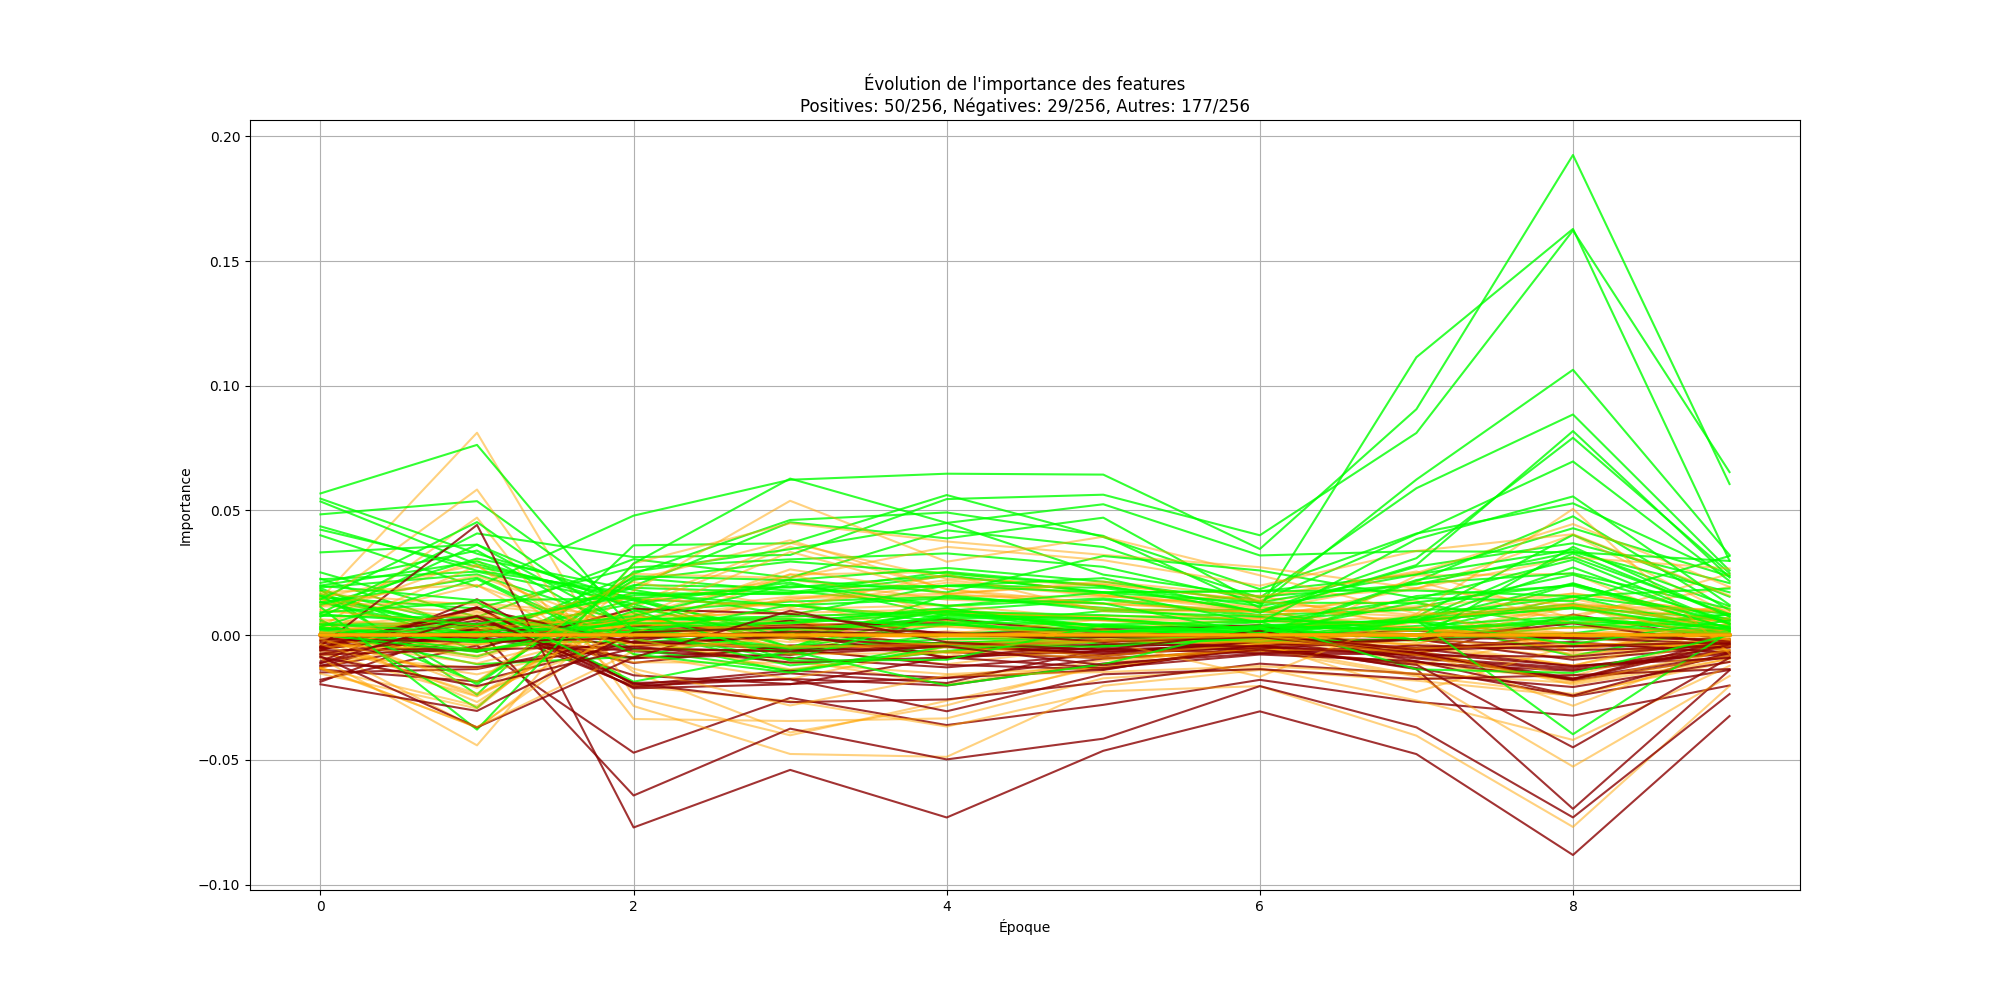
\includegraphics[width=\textwidth]{graphevolution.png}
\caption{Evolution de l'importance des features sur Ciphar-100 avec le model VGG-16 ImageNet} \label{fig1}
\end{figure}


Ainsi, afin de mieux adapter le réseau aux caractéristiques propres de CIFAR-100, nous avons entrepris de concevoir un modèle sur mesure en appliquant les mêmes principes de suppression des cartes d’activation.Toutefois, les résultats de cette nouvelle approche se sont avérés tout aussi peu concluants. L’analyse des activations a montré que la stabilité des cartes d’activation était insuffisante pour justifier leur suppression progressive, tout comme dans le cas précédent. Une même carte d’activation pouvait avoir un impact positif lors d'une époque, puis devenir négative à l'époque suivante. Cette fluctuation constante rendait difficile l'identification de motifs stables sur le long terme, rendant cette méthodologie peu exploitable en pratique. Ce constat souligne la complexité inhérente à la dynamique d'apprentissage des réseaux de neurones profonds, où les ajustements des poids à chaque itération peuvent entraîner des réorganisations significatives des activations. Néanmoins, cette piste de recherche reste intéressante et pourrait être approfondie en explorant des techniques complémentaires, comme la régularisation des activations ou l’utilisation de critères d’importance pondérés par la stabilité temporelle des cartes d'activation.

Dans la section suivante, nous détaillerons la méthode employée pour regrouper les cartes d'activation similaires en clusters. Ce regroupement vise à maximiser la cohérence des caractéristiques partagées entre différentes classes, tout en poursuivant notre objectif d’amélioration de l’explicabilité et de l’efficacité du modèle.

\subsection{Analyse de la robustesse des cartes d'activation à travers les cartes de chaleur}

En parallèle de l’évaluation de l’importance des cartes d'activation, nous avons mené une étude approfondie visant à mieux comprendre la robustesse et la cohérence des activations des cartes d'activation à travers différentes images. L’objectif principal de cette analyse était de déterminer dans quelle mesure une carte d'activation détectant un concept spécifique, tel qu’un œil sur une image, pouvait également identifier ce même concept sur d’autres images d’animaux, et comment elle se comportait lorsqu’un tel concept était absent. Pour ce faire, nous avons sélectionné plusieurs images d’animaux aux caractéristiques variées, incluant des espèces présentant des éléments anatomiques bien distincts (ex. : yeux visibles, nageoires, cornes) et d’autres où ces éléments sont soit dissimulés, soit absents. L’analyse s’est concentrée sur l’observation des cartes de chaleur générées pour chaque carte d'activation, permettant de visualiser les zones de l’image activées par le modèle.Les premières expérimentations ont révélé la capacité du réseau à identifier des concepts communs à travers différentes images. Par exemple, certaines cartes d'activation ont systématiquement activé des zones correspondant aux yeux ou aux nageoires lorsque ces éléments étaient présents sur l’image. Cette stabilité est essentielle pour la robustesse du modèle, car elle témoigne de la capacité des cartes d'activation à capturer des concepts universels plutôt que des détails propres à une seule image.

Cependant, lorsque le concept visé était absent de l’image, les résultats ont montré une grande variabilité. Dans certains cas, les cartes de chaleur demeuraient presque vides, avec des valeurs proches de zéro, indiquant l’absence d’activation significative. Dans d’autres situations, des régions aléatoires de l’image étaient activées, bien que ces activations restaient généralement de faible intensité comparées à celles observées pour des concepts réellement présents. Cette disparité met en évidence la difficulté pour le modèle de rester totalement inactif en l’absence de son concept cible, bien que les activations résiduelles ne soient généralement pas assez fortes pour perturber la classification globale.

Pour évaluer plus rigoureusement la résistance des cartes d'activation à la variabilité des images, nous avons introduit des perturbations visuelles. Nous avons notamment testé des images d’animaux dont les yeux sont partiellement ou entièrement dissimulés par des motifs de couleur ou des zones sombres. Parmi les espèces choisies figuraient l’orque, le panda et le hibou, dont les particularités visuelles posent des défis spécifiques.Les résultats ont montré des comportements contrastés :
\begin{itemize}
    \item Pour la classe hibou, les cartes de chaleur ont correctement détecté la position des yeux, démontrant la capacité du modèle à identifier des concepts même en présence de motifs complexes autour de la zone d’intérêt.
    \item Pour les classes panda et orque, contrairement à la classe hibou, les activations pour ces animaux se sont concentrées sur des zones de couleur unie, correspondant aux larges taches noires entourant la tête. Bien que ces activations ne ciblaient pas directement les yeux, elles mettaient en valeur le contour de ces zones, suggérant que le modèle assimilait parfois des motifs visuels globaux (comme une tache sombre) à des concepts localisés (comme un œil).
\end{itemize}
Cette différence de comportement soulève une question importante sur la nature des cartes d'activation extraites. Si, dans notre cas, la reconnaissance globale de l’animal n’est pas affectée par ce type de confusion (puisque le modèle reste capable d’identifier l’espèce indépendamment de la localisation précise des yeux), cela pourrait devenir problématique dans des applications nécessitant une identification fine des détails anatomiques. Par exemple, dans des contextes médicaux ou industriels, une mauvaise localisation d’un élément critique pourrait entraîner des erreurs d’interprétation.

Pour renforcer l’analyse, nous avons mesuré l’intensité moyenne des activations sur des zones cibles et hors cibles. Cette quantification a confirmé que, même lorsque le concept n’était pas correctement identifié, les activations restaient significativement plus faibles que celles observées lors de la détection correcte d’un concept. Cela suggère que, malgré certaines confusions visuelles, le modèle conserve globalement une hiérarchie d’importance entre les cartes d'activation activées.

Enfin, ces observations mettent en lumière l’importance de l’explicabilité dans les modèles d’apprentissage profond. Bien que les réseaux de neurones puissent parvenir à des résultats impressionnants en termes de précision brute, comprendre comment et pourquoi certaines activations se produisent reste crucial pour leur déploiement en toute confiance. Cette analyse de robustesse, combinée aux expérimentations sur les clusters de cartes d'activation, constitue un pas supplémentaire vers des réseaux plus interprétables et adaptés aux besoins spécifiques des utilisateurs.

\subsection{Création de superclasses}

Afin d’approfondir la compréhension des concepts appris par le modèle et d’améliorer la cohérence des cartes d'activation, nous avons entrepris la création de superclasses hiérarchiques à partir d’ImageNet. L’objectif de cette approche était de regrouper des catégories d’animaux partageant des caractéristiques visuelles communes. Une organisation par superclasses facilite l’analyse des concepts récurrents (ex. : yeux, pattes, cornes) et leur généralisation sur différentes espèces. Pour structurer cette hiérarchie, nous avons défini trois grandes superclasses basées sur les milieux naturels :
\begin{itemize}
    \item Terrestre : incluant des sous-classes comme les animaux à cornes, les quadrupèdes ou encore les primates.
    \item Aérien : regroupant notamment les oiseaux planeurs, les rapaces et les chauves-souris.
    \item Aquatique : contenant des sous-classes telles que les mammifères marins et les poissons.
\end{itemize}
La création de ces superclasses a nécessité la constitution d’un dataset personnalisé dérivé d’ImageNet. Nous avons utilisé un code existant pour extraire les images correspondant aux classes visées. Cependant, ce code initial présentait des incompatibilités avec les versions récentes de certaines bibliothèques. Nous l’avons donc adapté en corrigeant les erreurs et en mettant à jour les dépendances pour garantir la compatibilité avec les outils actuels. Cette étape de nettoyage et d’actualisation a été essentielle pour assurer la qualité et la fiabilité des données utilisées.

\subsection{Identification des concepts communs via le regroupement des cartes d'activation}

Avec le nouveau dataset constitué, notre objectif suivant était de regrouper les cartes d'activation en fonction des concepts visuels qu’elles représentaient. Nous nous sommes particulièrement intéressés à des concepts visuellement saillants et fréquemment rencontrés tels que les "yeux", les "pattes", les "cornes" ou encore la "zone ventrale" des animaux. Pour réaliser ce regroupement, nous avons appliqué différentes méthodes de regroupement sur les cartes de chaleur générées par le modèle.

Dans un premier temps, nous avons testé plusieurs algorithmes de regroupement directement sur les cartes de chaleur brutes. Ces premières expérimentations se sont révélées peu concluantes. La principale difficulté résidait dans l’amplitude variable des valeurs d’une carte de chaleur à l’autre : un point fortement activé sur une image pouvait avoir une valeur de 1, tandis qu’un point tout aussi important sur une autre image atteignait seulement 0,1. Cette disparité biaisait les regroupements et rendait l’identification de concepts communs imprécise. Pour pallier ce problème, plusieurs prétraitements ont été appliqués aux cartes de chaleur :
\begin{itemize}
    \item Valeur absolue : Chaque valeur de la carte de chaleur a été transformée en sa valeur absolue, garantissant que les activations négatives et positives contribuent de manière équivalente à l’analyse. L’objectif était de mettre en évidence l’importance d’un point, indépendamment du signe de son activation.
    \item Normalisation min-max : Pour uniformiser les amplitudes, chaque carte de chaleur a été normalisée entre 0 et 1. Ainsi, le point le plus activé avait systématiquement une valeur de 1 et le moins activé une valeur de 0. Cette étape a permis d’éliminer les biais liés aux variations d’échelle et de comparer équitablement les activations entre différentes images. L’objectif de la normalisation par min-max était d’empêcher les algorithmes de regroupement de classifier les images uniquement en fonction des valeurs absolues des activations. Ce prétraitement visait à contraindre ces algorithmes à se baser plutôt sur la répartition et l’écart relatif entre les valeurs d’une carte de chaleur.
\end{itemize}
Ces transformations ont significativement amélioré la lisibilité et la pertinence des regroupements obtenus par la suite.

Parmi les méthodes testées, l’algorithme KMeans s’est montré le plus performant pour notre problématique. Nous avons appliqué KMeans avec un nombre de clusters variant de 2 à 15 afin d’observer l’évolution des regroupements et d’identifier la configuration la plus adaptée, visibles sur la figure \ref{fig2}.

\begin{figure}
\centering
\setlength{\abovecaptionskip}{2pt} % Réduit l'espace avant la légende
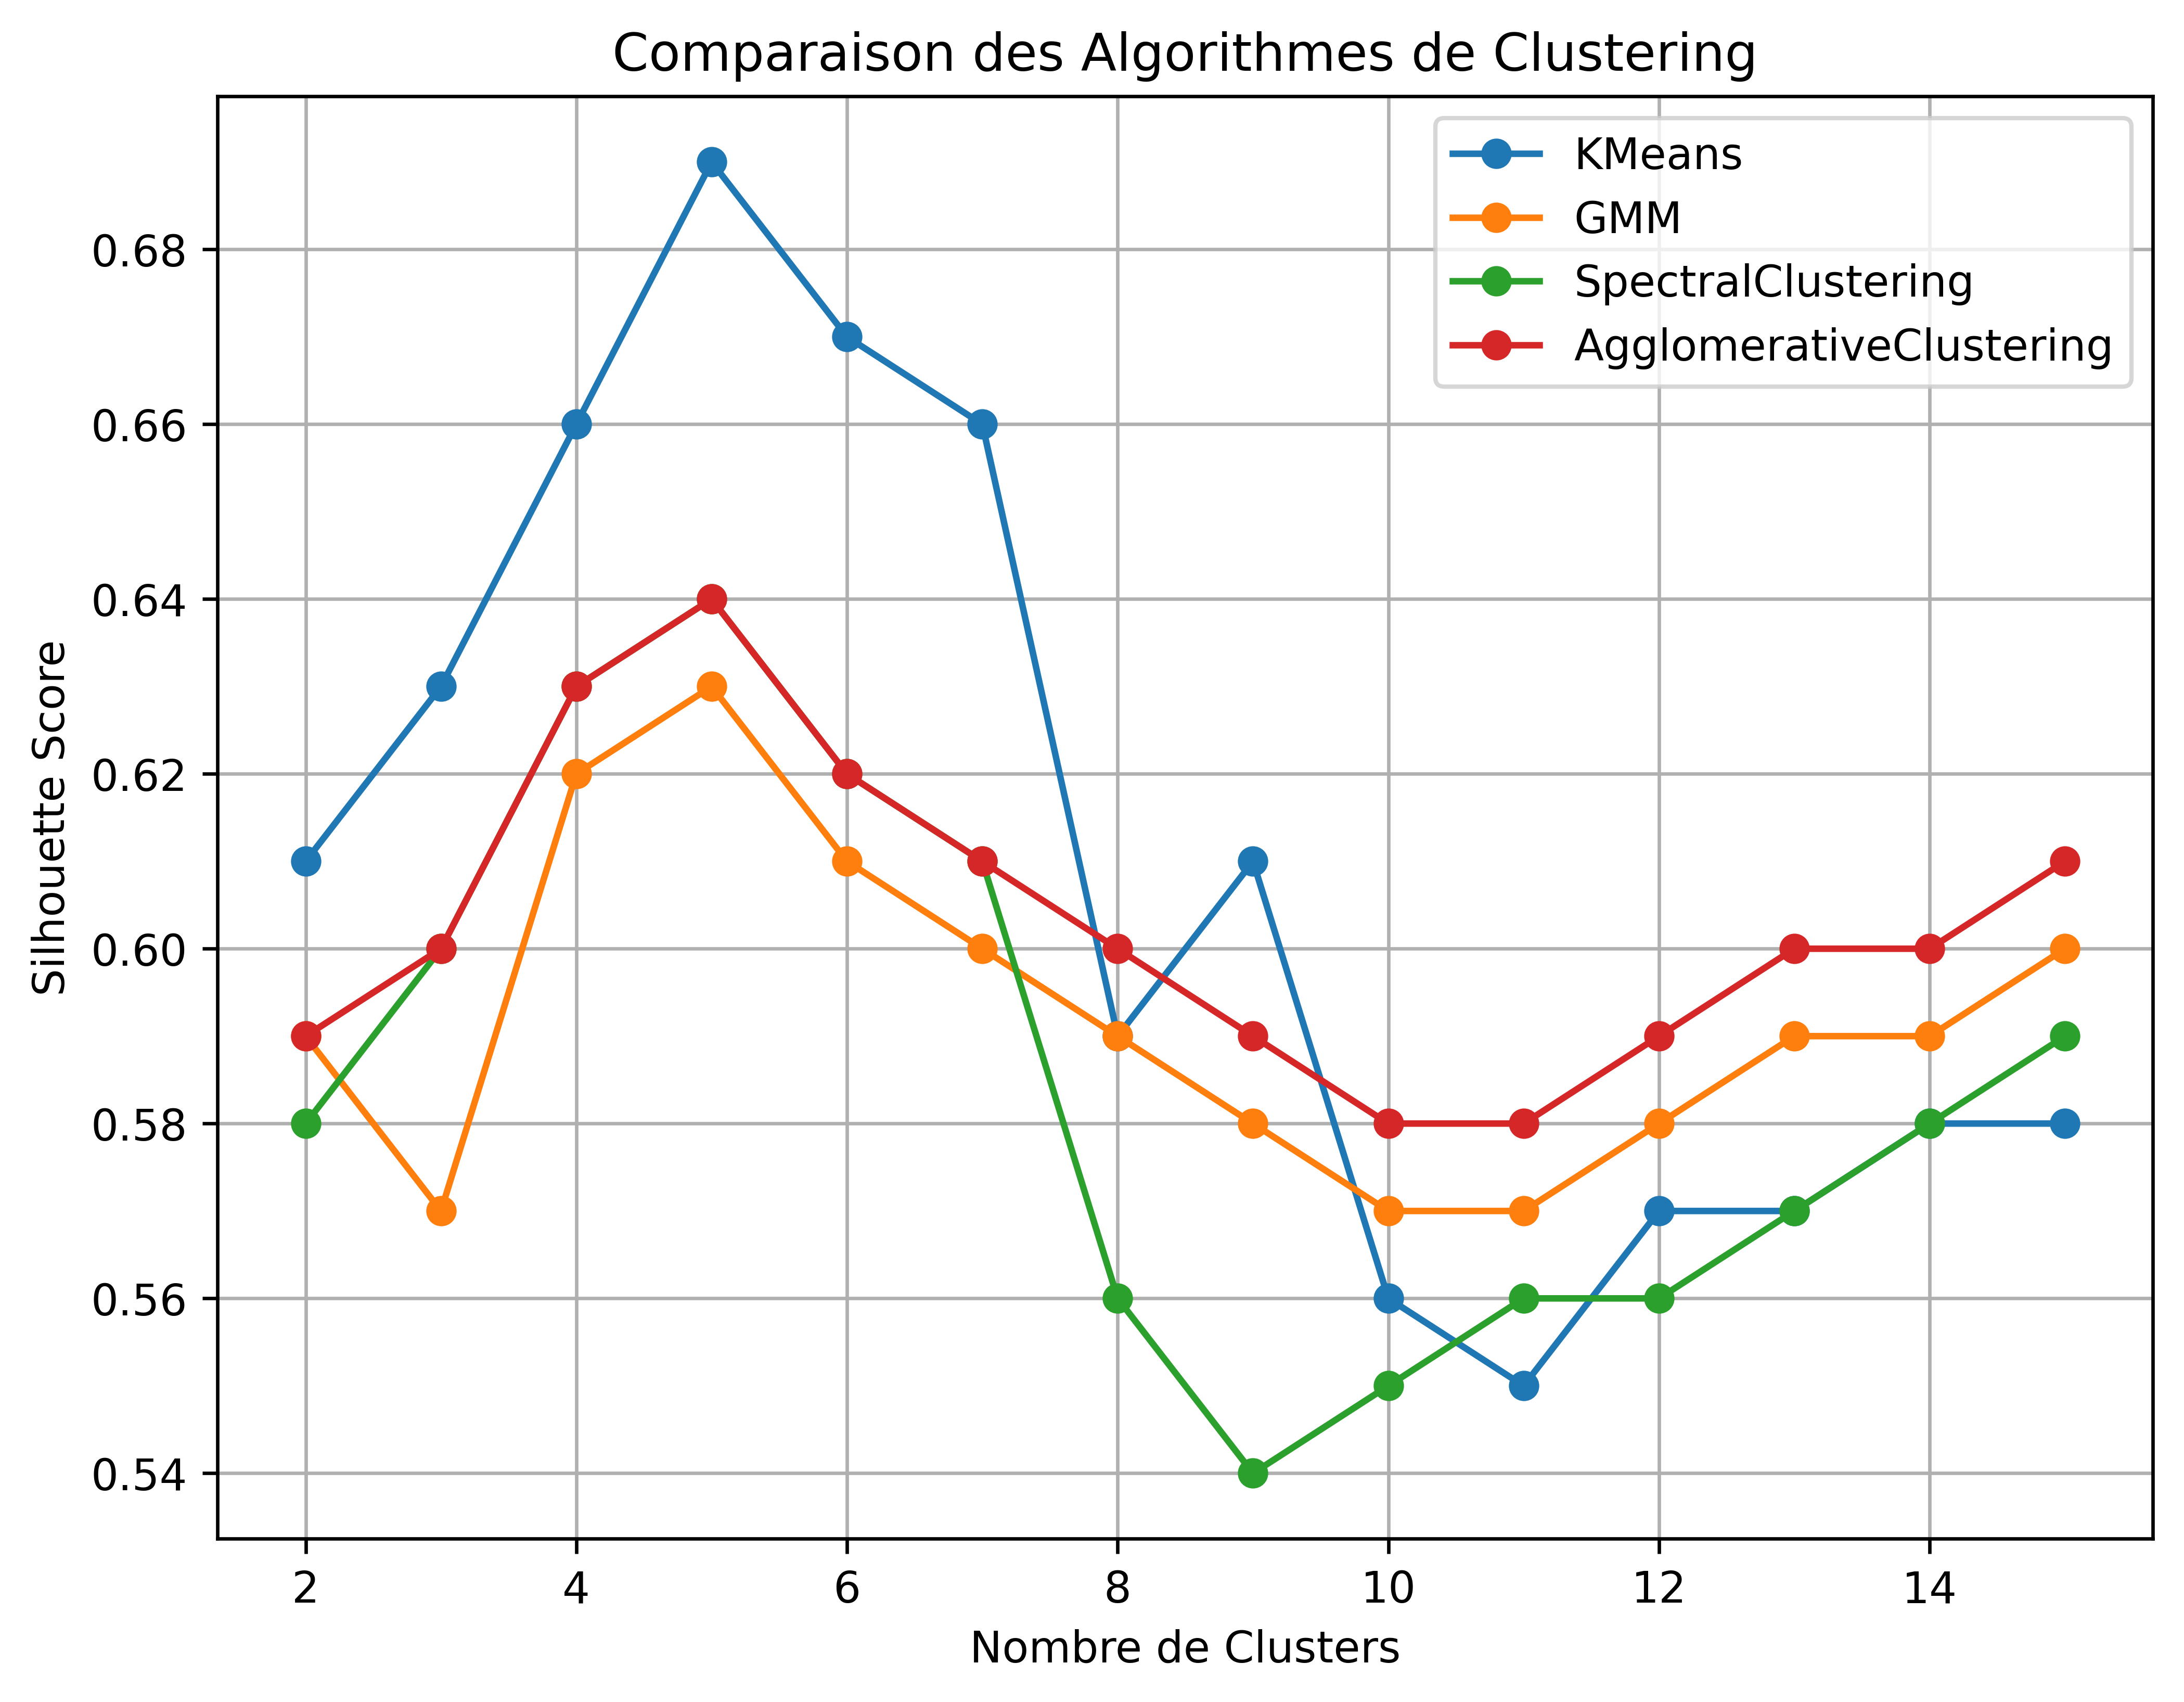
\includegraphics[scale=0.4]{clustering_comparaison.png}
\caption{Évolution des performances de différentes techniques de regroupement en fonction du nombre de clusters souhaité} \label{fig2}
\end{figure}

Les résultats ont montré que :
\begin{itemize}
    \item Sur des images focalisées sur une partie spécifique de l’animal (ex. : gros plan sur la tête ou une patte), un nombre restreint de clusters (2 à 5) suffisait à isoler des concepts pertinents.
    \item Sur des images montrant l’animal en entier, un nombre de clusters plus élevé (10 à 15) permettait de mieux segmenter les différentes régions anatomiques.
\end{itemize}
Ces observations confirment que le niveau de détail de l’image influence directement la granularité nécessaire pour une segmentation efficace.
Dans un second temps, une annotation des différents clusters a été réalisée afin d’évaluer leur pertinence. Il est apparu que, dans certains cas, le nombre de clusters obtenus était supérieur au nombre de concepts réellement présents. Autrement dit, nous avons observé des clusters supplémentaires correspondant à des zones non interprétables. Par exemple, pour une image donnée, trois clusters ont été identifiés et annotés comme suit : le premier représentait les yeux, le second les cornes et le troisième n’était pas exploitable en raison de valeurs trop faibles, et a donc été labellisé comme « None ». Afin d’améliorer la qualité des résultats et d’éviter les biais liés à la nature des images traitées, nous avons étendu l’analyse à un ensemble plus varié d’images. Plutôt que de nous limiter à des vues frontales, nous avons intégré des images présentant l’animal sous différents angles (de profil, de dos, en groupe, en gros plan, etc.). Cette diversification visait à accroître la robustesse des résultats en prenant en compte une plus grande variabilité des formes et des perspectives. Une fois ces données collectées, nous avons croisé les activations neuronales associées aux différents clusters pour affiner l’attribution des activations à un cluster spécifique. La méthodologie adoptée consistait à comptabiliser la fréquence d’apparition d’une activation neuronale donnée au sein des clusters, comme on peut l’observer sur l’image de gauche de la figure \ref{fig3}. Par exemple, si une activation neuronale apparaissait 10 fois dans un cluster « œil », 5 fois dans le cluster « None » et 8 fois dans le cluster « cornes », elle était alors attribuée au cluster « œil », correspondant à la catégorie la plus représentée.

\begin{figure}
    \centering
    \setlength{\abovecaptionskip}{2pt} % Réduit l'espace avant la légende
    \begin{minipage}{0.49\linewidth}
        \centering
        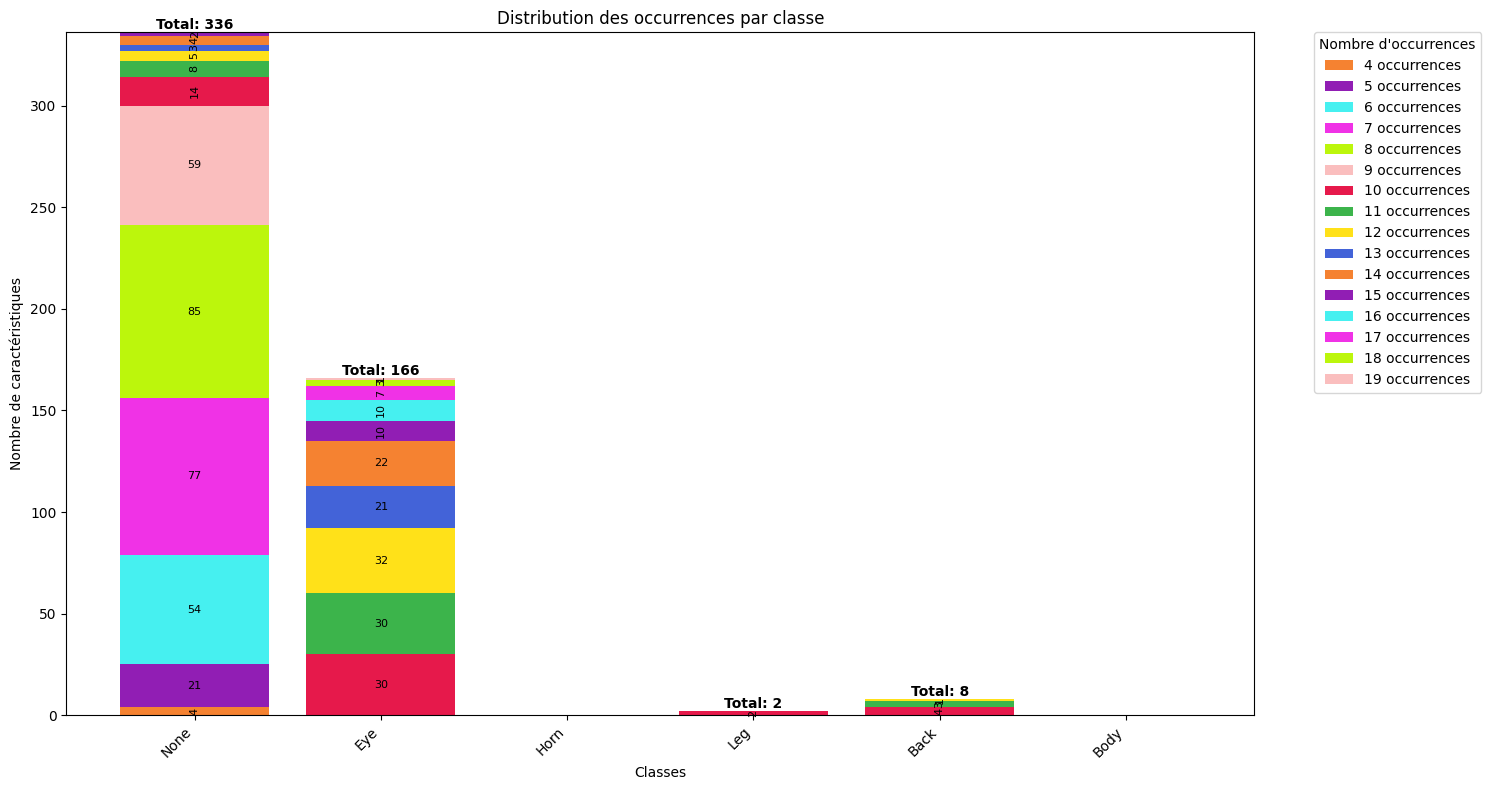
\includegraphics[width=\linewidth]{barPERnul.png}
    \end{minipage}%
    \hfill
    \begin{minipage}{0.49\linewidth}
        \centering
        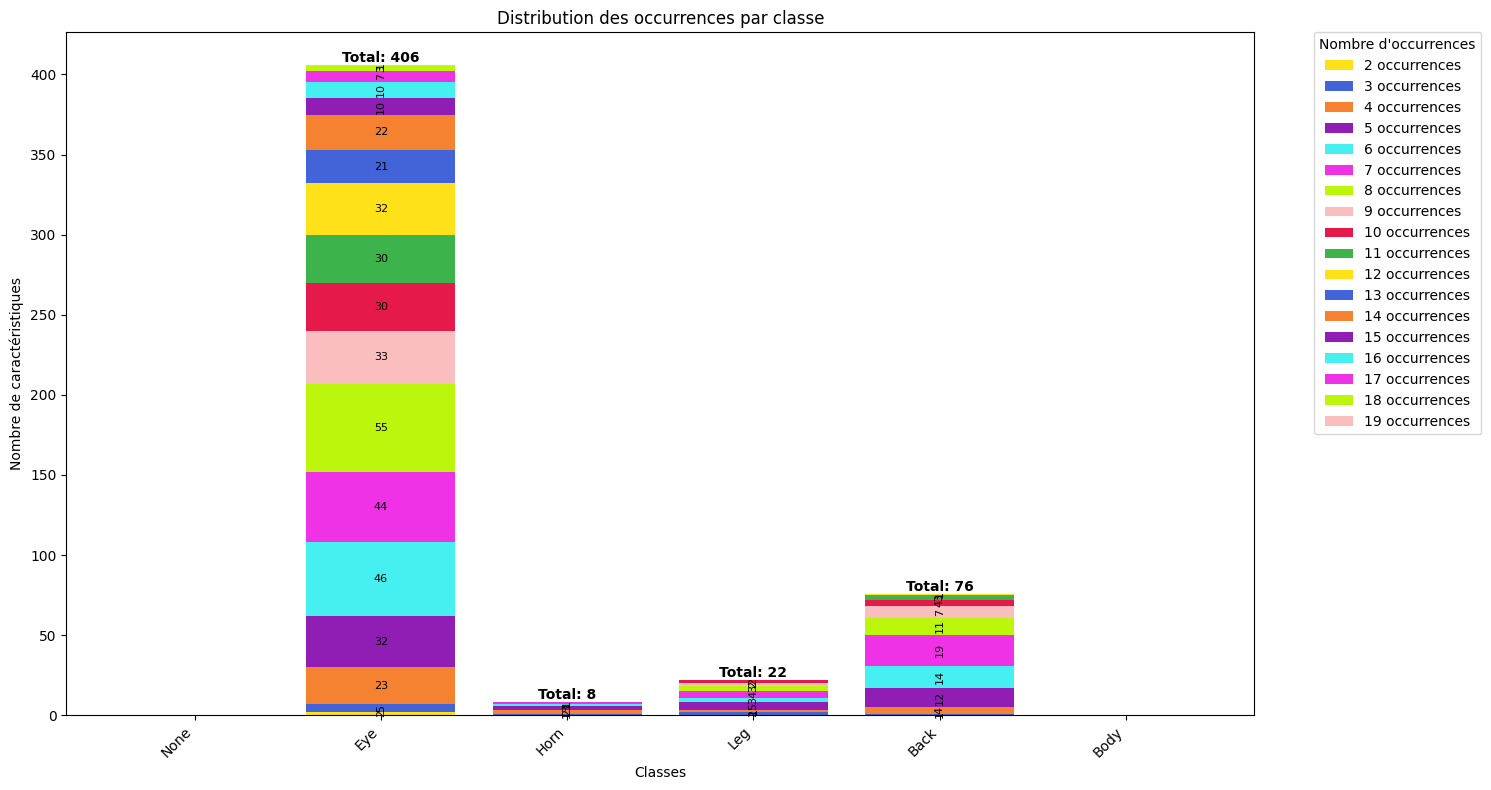
\includegraphics[width=\linewidth]{barPER.png}
    \end{minipage}
    \caption{Visualisation des clusters des activations neuronales de 25 images. À gauche, croisement des cartes d’activation avec le cluster 'None'. À droite, même représentation en utilisant le deuxième cluster le plus présent après 'None'}
    \label{fig3}
\end{figure}

Cependant, cette approche initiale a révélé certaines limites. En effet, nous avons constaté que le cluster « None » avait tendance à devenir majoritaire, réduisant ainsi la pertinence des autres clusters. Cette situation était directement liée au faible nombre d’images analysées (25 images traitées à ce stade). La quantité limitée de données disponibles a conduit à une surreprésentation du cluster « None », notamment en raison de l’absence de certains concepts dans plusieurs images, faussant ainsi l’équilibrage global. Nous avons estimé qu’un nombre minimal de 100 images distinctes serait nécessaire pour obtenir des résultats plus fiables et représentatifs. Toutefois, en raison des contraintes de temps imposées par le calendrier, nous avons ajusté notre méthodologie d’affectation des activations neuronales. Désormais, le cluster « None » ne peut plus être considéré comme dominant. Ainsi, lorsqu’un cluster est identifié comme majoritaire mais correspond à « None », nous réattribuons les activations neuronales au cluster significatif le plus représenté après celui-ci. Cette modification a eu un impact immédiat : les résultats obtenus ont montré une meilleure répartition des activations neuronales, permettant de faire émerger des clusters pertinents tels que « cornes » ou « pattes », comme illustré sur l’image de droite de la figure \ref{fig3}.



Cette nouvelle approche a donc amélioré la segmentation des différentes régions anatomiques de l’animal et renforcé la cohérence des annotations, tout en atténuant l’effet de sous-représentation lié au faible nombre d’images initialement traitées. Les différents clusters ont été testés sur plusieurs images et classes inconnues lors de l’entraînement, et les résultats sont convaincants. Ainsi, les cartes de chaleurs résultantes mettent bien en évidence les différents concepts, comme on peut le voir sur la figure \ref{fig4}. 

\begin{figure}
\centering
\setlength{\abovecaptionskip}{2pt} % Réduit l'espace avant la légende
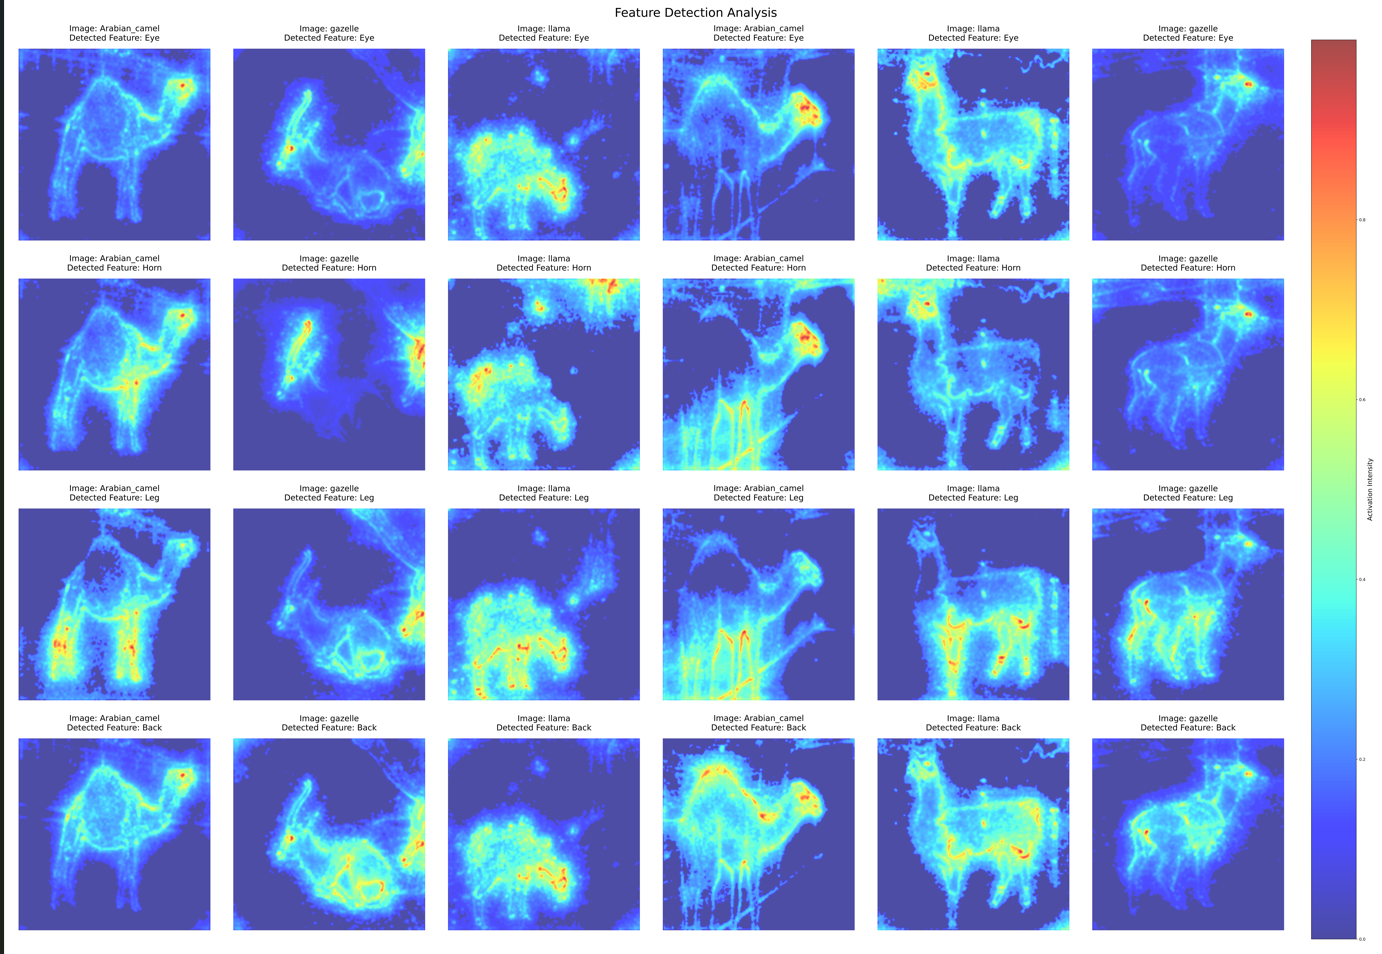
\includegraphics[scale=0.2]{resultats.png}
\caption{Clusters des concepts "Oeil", "Cornes", "Pattes" et "Dos" créés sur 25 images de gazelles et appliquées à plusieurs images} \label{fig4}
\end{figure}

\subsection{Double-regroupement et automatisation du regroupement de concepts}

Bien que la méthode précédente ait permis de détecter efficacement certains concepts, elle reposait encore sur une annotation manuelle des clusters, ce qui pouvait s’avérer long et sujet à des biais. Pour surmonter cette limite et automatiser le processus tout en cherchant à améliorer la robustesse des résultats, nous avons mis en place une stratégie de double-regroupement. Cette approche consiste à appliquer l’algorithme de regroupement en deux étapes successives :
\begin{enumerate}
    \item Premier regroupement par image : Pour chaque image, nous avons appliqué KMeans sur les activations neuronales. Cette étape permet de regrouper localement les activations correspondant à des concepts spécifiques à l’image (ex. : les activations correspondant aux yeux ou aux pattes sur cette image précise).
    \item Second regroupement sur les clusters obtenus : Une fois les clusters extraits de chaque image, nous avons réappliqué un algorithme de regroupement sur l’ensemble de ces groupes. Ce second niveau, que nous appelons super-regroupement, vise à fusionner les clusters similaires provenant d’images différentes, sans intervention humaine directe pour les annoter. Pour mettre en œuvre cette étape, chaque cluster a été converti en un vecteur binaire de 512 dimensions, où chaque dimension correspond à une caractéristique spécifique, prenant la valeur 1 si la caractéristique est présente dans le cluster et 0 sinon.
\end{enumerate}
Ce processus permet de regrouper automatiquement des concepts communs entre les images. Par exemple, un cluster identifié comme représentant un œil sur une image devrait être regroupé avec d’autres clusters similaires provenant d’images différentes, formant ainsi un méta-cluster stable et représentatif du concept "œil". En réduisant la variance entre les images, cette méthode facilite l’émergence de concepts globaux et cohérents. Une difficulté rencontrée lors de cette étape concernait les activations proches mais correspondant à des concepts différents. Sans précaution, une activation détectée sur une image pouvait être indûment rapprochée d’une autre, activée dans un contexte visuel différent. Grâce au double-regroupement, ces erreurs ont été réduites, car le second niveau de regroupement privilégie la stabilité des activations sur plusieurs images et non les proximités accidentelles observées sur une seule. \newline
\indent L’évaluation préliminaire des big-clusters a montré des tendances intéressantes, bien que les résultats ne puissent être considérés comme concluants en raison du nombre limité d’images traitées. Les concepts "yeux", "pattes", "cornes" et "corps/ventre" semblaient être correctement regroupés dans les premiers tests, suggérant une certaine généralisation des concepts entre différentes images. Cependant, faute d’un volume d’images suffisant, il n’a pas été possible de vérifier pleinement la robustesse du double-regroupement. Par ailleurs, certains big-clusters annotés comme "None" sont restés difficiles à interpréter. Ceux-ci pourraient correspondre à des concepts visuels latents non présents dans nos annotations initiales (ex. : nageoires, structures d’objets comme des portes ou des fenêtres), mais faute de données avec des clusters annotées suffisantes, nous n’avons pas pu approfondir leur analyse. Cette limitation souligne la nécessité d’un ensemble de données annotées plus large pour mieux comprendre l’impact de cette approche.

\section{Conclusion et perspectives}

\subsection{Conclusion}

En somme, notre recherche s'est articulée autour de plusieurs axes méthodologiques visant à améliorer l'explicabilité des réseaux de neurones convolutifs, en particulier dans le contexte de la classification d'images.

Nous avons d'abord reproduit avec succès les résultats du Concept Relevance Propagation (CRP) \autocite{Achtibat2023} et de sa variante Layer-wise CRP (L-CRP) \autocite{inproceedings}. Cette phase a permis de valider notre compréhension des approches existantes et d'établir une base solide pour nos expérimentations. La génération des cartes de chaleur illustrant l'activation des différentes couches a confirmé la fiabilité de notre implémentation et constitué le socle de notre démarche expérimentale.

L'analyse des cartes obtenues avec VGG16 préentraîné sur ImageNet a révélé une progression cohérente des caractéristiques extraites : les premières couches captent des contours et textures, tandis que les couches plus profondes, notamment la couche 40, détectent des concepts anatomiques précis (yeux, ailes, pattes). Cette évolution hiérarchique valide notre approche d'analyse.

L'évaluation des cartes d'activation a produit des résultats intéressants. En désactivant individuellement chaque carte et en observant la variation du score de prédiction, nous avons identifié les cartes "utiles", "inutiles" ou "négatives". En conservant uniquement les cartes positives, la précision atteignait 98\% sur certaines images, contre 78\% initialement, tandis que l'utilisation exclusive des cartes négatives faisait chuter la précision à des valeurs proches de zéro. Ces résultats suggèrent qu'une sélection judicieuse des cartes d'activation pourrait optimiser les performances du modèle.

Toutefois, nos tentatives d'optimisation du réseau ont produit des résultats contrastés. L'approche consistant à désactiver les cartes jugées inutiles s'est avérée prometteuse sur un sous-ensemble d'ImageNet, mais moins efficace sur CIFAR-100, probablement en raison de la spécificité de l'architecture VGG16 et de l'instabilité des cartes d'activation. Ces résultats soulignent la complexité de l'apprentissage des réseaux profonds et appellent à une approche plus nuancée de l'optimisation.

L'analyse de la robustesse des cartes d'activation a révélé des comportements variables selon les concepts et images. Certaines cartes identifiaient systématiquement des concepts comme les yeux, tandis que d'autres montraient plus de variabilité en cas de concepts absents ou partiellement visibles. Bien que cela n'affecte généralement pas la classification globale, cela soulève des questions sur la fiabilité des cartes dans des contextes nécessitant une précision anatomique fine.

Enfin, notre approche de double-regroupement pour l'identification automatique des concepts visuels constitue l'innovation finale de notre travail. En appliquant un regroupement à deux niveaux, nous avons cherché à faire émerger des concepts stables sans annotation manuelle extensive. Les premières évaluations ont montré un regroupement cohérent de concepts comme les "yeux", "pattes" ou "cornes", mais le nombre limité d'images traitées n'a pas permis de valider pleinement la robustesse de cette approche. Une validation à plus grande échelle reste nécessaire.

\subsection{Perspectives}

Ces résultats ouvrent plusieurs axes de recherche pour prolonger et approfondir notre travail.

Le double-regroupement représente une avancée conceptuelle vers l'automatisation de l'identification des concepts visuels tout en limitant les biais liés à l'annotation manuelle. Cette approche mériterait d'être étendue à un corpus d'images considérablement plus vaste, idéalement plusieurs centaines voire milliers d'images, afin d'en évaluer pleinement l'efficacité et la robustesse. Une telle validation à grande échelle permettrait non seulement de confirmer la pertinence des concepts identifiés, mais également d'explorer l'émergence de concepts visuels plus subtils ou spécifiques à certaines catégories d'images.

L'instabilité observée dans les cartes d'activation au cours de l'apprentissage suggère l'intérêt d'explorer des techniques de régularisation spécifiquement conçues pour stabiliser ces activations. Des mécanismes de régularisation temporelle, qui pénaliseraient les fluctuations abruptes des activations d'une époque à l'autre, pourraient contribuer à renforcer la cohérence et la fiabilité des concepts extraits. Cette stabilisation faciliterait grandement l'interprétation des décisions du modèle et améliorerait potentiellement ses performances.

L'identification de cartes d'activation redondantes ouvre également la voie à des méthodes de compression de réseaux plus efficientes. En détectant systématiquement les redondances fonctionnelles au sein du modèle, il serait possible de concevoir des architectures plus légères sans sacrifier les performances. Cette approche pourrait s'avérer particulièrement pertinente pour le déploiement de modèles sur des dispositifs à ressources limitées, comme les applications mobiles ou embarquées.

Enfin, l'intégration des connaissances issues de notre analyse dans des systèmes d'explicabilité plus complets constitue une perspective particulièrement stimulante. Les concepts visuels identifiés pourraient être associés à des descriptions sémantiques, permettant ainsi de générer des explications en langage naturel des décisions du modèle. Un tel système d'explicabilité multimodale faciliterait considérablement l'interaction entre les utilisateurs non experts et les modèles d'intelligence artificielle, contribuant ainsi à renforcer la confiance dans ces technologies. 

\printbibliography

\end{document}
